%% ------------------------------------------------------------------------- %%
\chapter{Test-Driven Development e Design de Classes}
\label{cap:tdd-e-design}

É comum relacionar TDD à práticas de testes de software. Mas, apesar de ter o
termo ``teste'' no nome, TDD não é uma prática de testes.
Apesar da criação de testes ser algo intrínseco ao processo, TDD é uma prática
que auxilia o desenvolvedor a desenhar classes mais flexíveis, mais coesas e
menos acopladas. Os testes são a ferramenta que o programador utiliza para
validar o design criado. Por esse motivo, muitos se referem a TDD como
\textit{Test-Driven Design}, ou seja, design guiado pelos testes
\cite{tdd-taxonomy}.

Um ponto interessante a ser notado é que nenhum livro sobre TDD \cite{GOOS}
\cite{TDDByExample} \cite{astels-tdd}, discute em momento algum qualquer
prática conhecida da área de testes de software, como análise do valor-limite ou
grafo de causa-efeito \cite{art-of-sw-testing}, o que leva a crer que os
benefícios de TDD não são os mesmos da área de testes.

Muitos autores como Kent Beck \cite{aim-fire}, Dave Astels \cite{astels-tdd} e
Robert Martin \cite{bob-martin} afirmam que TDD é na verdade uma prática de
design \cite{tdd-taxonomy} \cite{aim-fire}.
Na opinião desses autores, a mudança na ordem do ciclo de
desenvolvimento tradicional, apesar de simples, agrega diversos outros
benefícios ao código produzido: simplicidade, foco, melhor design, entre outras.
Ward Cunningham, um dos pioneiros da Programação Extrema resume essa discussão
em uma simples frase: \textit{Test-First programming is not a testing technique}
que, em uma tradução livre, significa \textit{Testar Primeiro não é uma prática 
de testes}.

O foco deste trabalho não é observar TDD sob esse ponto de vista, mas muitos
outros estudos avaliam TDD sob esse ponto de vista e podem ser encontrados na
seção \ref{cap:trabalhos-relacionados}.

%% ------------------------------------------------------------------------- %%
\section{Definições incompletas}

Apesar do foco da prática em design, é possível encontrar muitas definições que
não levam isso em conta. Algumas delas levam em consideração apenas a ideia da
inversão da ordem de desenvolvimento, aonde o programador deve primeiro escrever
o teste e depois escrever o código que faça o teste passar.

Um exemplo disso é a definição que pode ser encontrada no livro \textit{JUnit
in Action} \cite{junit-in-action}: \textit{Test-Driven Development é uma
prática de programação que instrui desenvolvedores a escrever código novo
apenas se um teste automatizado estiver falhando, e a eliminar duplicação. O
objetivo de TDD é "código claro que funcione"}.

Apesar de ser correta, ela é incompleta, já que ela não captura a parte mais
interessante da prática, que é feedback no design. Janzen também levanta esse
problema e culpa até o próprio nome da prática, já que ela possui a palavra
``testes'', mas não contém a palavra ``design'' \cite{tdd-really-improve}.

Uma definição mais clara é a de que TDD é a arte de produzir testes
automatizados para código de produção, usando esse processo para guiar o design e a programação.
Para cada pequeno pedaço de funcionalidade, o desenvolvedor deve primeiro
escrever um teste que especifique e valide o que o código irá fazer. O
programador então produz somente o código necessário para fazer esse teste
passar. Então ele refatora (simplifica e clareia) tanto o código de produção
quanto o código de testes \cite{agilealliance-tdd} \cite{tdd-taxonomy}.

Muitos dos artigos utilizados na escrita dessa dissertação apresentam definições
de TDD que não levam em conta seus efeitos no design, e talvez por isso muitas das 
pesquisas em relação à prática avaliam os efeitos de TDD sobre a qualidade 
externa, algo geralmente avaliado em técnicas de testes. Esses estudos são 
explicados com mais detalhes no capítulo \ref{cap:trabalhos-relacionados}.

%% ------------------------------------------------------------------------- %%
\section{Efeitos no design}

Na abordagem tradicional, programadores escrevem boa parte do código antes de
testarem. Ao perceberem posteriormente um problema no design, o preço para
corrigir pode ser alto demais. Uma vantagem de escrever os testes antes é
possibilitar que o desenvolvedor tome grande parte das decisões de design
enquanto o custo de mudança ainda é baixo.

O teste é o primeiro cliente da
classe que o programador ainda está por escrever e isso faz com que ele pense
melhor a respeito do comportamento que ele espera da classe. Além disso,
programadores contemplam e decidem também sobre a interface (como nomes de
classes e métodos, tipos de retorno e exceções lançadas) que a classe terá
\cite{janzen-saiedian}.
Além disso, ao escrever o teste antes, o programador é encorajado a escrever um
código que seja facilmente testável. Códigos como esse possuem algumas
características interessantes, como a facilidade para invocar o comportamento
esperado, a não necessidade de pré-condições complicadas e a explicitação de
todas as dependências que a classe possui.

Gerenciamento de dependências que, conforme comentado por Robert Martin em uma
de suas palestras \cite{bobmartin-infoq}, é uma das partes mais delicadas de
todo o processo de desenvolvimento de software. Quando as dependências são mal
gerenciadas, o código torna-se difícil de manter, de evoluir e de se reutilizar.
Alterações simples demandam grandes alterações no código, já que elas se
propagam por diversas outras classes do sistema.
TDD reduz esses problemas já que, para escrever um teste de unidade para uma
determinada classe que colabora com outra, essa classe deve ter suas
dependências explícitas e deve permitir que a implementação do colaborador seja
trocada a qualquer momento. Se isso não for feito, o programador não conseguirá
testar aquela unidade de maneira isolada; ele vai sempre depender da execução da
dependência.

Quanto mais difícil for a escrita do teste, maior a chance da existência de
algum mau cheiro de design. Segundo Michael Feathers, existe uma sinergia muito
grande entre uma classe com alta testabilidade e um bom design: se o
programador busca por testabilidade, ele acaba criando um bom design; se o
programador busca por um bom design, ele acaba escrevendo um design mais
testável \cite{feathers-synergy}.

Classes altamente acopladas, além de difíceis de manter, também são difíceis de
testar, já que o programador deverá fazer uso de muitos objetos dublês para
simular o comportamento esperado das dependências.
O teste pode dar ainda muitos outros feedbacks sobre a qualidade do design,
além do acoplamento. Uma classe que possui muita responsabilidade (ou seja, é
pouco coesa) é também difícil de testar, já que o programador gastaria muito
tempo testando todas as possíveis possibilidades. Esse tipo de classe geralmente
apresenta código complexo. Nesse caso, o programador praticante de TDD, ao
enxergar a dificuldade da escrita do teste, refatoraria a mesma, quebrando-a em
pequenas classes.

TDD encoraja o programador a escrever componentes fracamente acoplados, de
maneira que eles possam ser testados de maneira isolada, e em um nível maior,
combinados com outros componentes.
Programar voltado para interfaces é uma prática de orientação a objetos há muito
tempo conhecida. A ideia de pensar em classes e dar mais foco à maneira com que
elas se relacionam do que com a maneira que elas implementarão determinado
algoritmo passa a ser natural \cite{GOOS}. 

%% ------------------------------------------------------------------------- %%
\section{Efeitos na Simplicidade}

TDD sugere que o programador dê sempre pequenos passos (conhecidos pelo termo em
inglês, \textit{baby steps}): deve-se escrever testes sempre para a menor
funcionalidade possível, escrever o código mais simples que faça o teste passar
e fazer sempre apenas uma refatoração por vez.

Uma justificativa para tal é que quanto maior o passo que o programador dá, mais
tempo ele leva para concluir esse passo e, consequentemente ele fica mais tempo
sem feedback sobre o código. Além disso, faz com que o programador não crie
soluções mais complexas do que elas precisam ser, tornando o código, à longo
prazo, o mais simples possível.

Em seu livro, Kent Beck dá exemplos de simplicidade, e na implementação de uma
operação de multiplicação dentro de uma simples classe \textit{Dinheiro},
responsável por representar uma unidade monetária, Beck escreve o seguinte
teste e implementação \cite{TDDByExample}:

\begin{lstlisting}[frame=trbl]
public void testaMultiplicacao() {
	Dinheiro cinco = new Dinheiro(5);
	cinco.vezes(2);
	assertEquals(10, dinheiro.valor);
}
	
class Dinheiro {
	public int valor = 10;
		
	Dinheiro(int valor) { }
		
	void vezes(int multiplicador) {}
}
\end{lstlisting}

Repare Beck fez o teste passar da maneira mais simples possível: fez o atributo
\textit{valor} receber diretamente o valor da multiplicação. E, somente com os
testes passando, Beck refatora e remove a duplicação de dados e de código
existente (o valor 10 é informação duplicada entre o teste e o código da
classe):

\begin{lstlisting}[frame=trbl]
class Dinheiro {
	public int valor;
	
	Dinheiro(int valor) {
		this.valor = valor;
	}
	
	void vezes(int multiplicador) {
		valor = valor * multiplicador;
	}
}
\end{lstlisting}

O teste ainda continua passando, provando que a refatoração foi feita com
sucesso. Pode-se observar através do exemplo acima que os passos dados foram
sempre os menores e mais simples possíveis, ou \textit{passos de bebê}, por
assim dizer. Veja que, mesmo após diversos passos de refatoração, ainda é
possível encontrar problemas de design, como o atributo \textit{valor}
declarado como público. Seriam necessários outras rodadas de refatoração para
eliminar esse problema.

Uma confusão comum de programadores que experimentam TDD pela primeira vez é a
de que fazer passos de bebê o tempo todo faz com que a produtividade diminua.
De fato, fazer passos de bebê durante todo o ciclo faz com que o tempo de
desenvolvimento aumente, já que muitos desses passos são simples demais e
poderiam ser pulados por um programador mais experiente. 

Mas TDD não força o programador a dar passos de bebê o tempo todo, mas sim
permite que o mesmo dê passos de bebê quando achar necessário
\cite{TDDByExample}: caso o programador esteja confiante sobre o trecho de
código  que está escrevendo naquele momento, ele pode dar um passo maior;  mas
caso ele não esteja tão confiante, a prática permite a ele ir mais devagar e 
dar passos de bebê, obtendo feedback mais rápido sobre o código que está
escrevendo.

O próprio Kent Beck em seu livro afirma que não faz passos tão pequenos o tempo
todo, mas se sente seguro em saber que pode dar passos pequenos quando houver
necessidade.

No exemplo acima, o método \textit{vezes} poderia ser considerado simples por
um programador experiente, que optaria por chegar à mesma solução acima de
maneira mais rápida, tomando passos maiores. Nesse momento, a experiência do
programador deve ditar o ritmo.

O conceito de simplicidade de TDD vai além da implementação de um método; a
simplicidade do design é algo também fundamental. Em modelos tradicionais de
desenvolvimento de software, diagramas de classe são criados para tentar prever
futuras alterações no software, colocando diversos pontos de flexibilização no
modelo. Muitas dessas previsões podem não se concretizar, deixando o design
desnecessariamente complexo.

Equipes ágeis optam por não fazer o chamado \textit{big design up-front (BDUF)},
e deixar que o design emerja ao longo do tempo, mantendo o código o mais claro e
simples possível, e refatorando sempre que há necessidade. Decisões de
design são tomadas com a consciência de que elas serão alteradas no futuro
\cite{is-design-dead}.

Manter o design simples não é tarefa fácil, e TDD sugere que o programador
escreva sempre o código mais simples que atenda a necessidade. Somente se a
necessidade crescer, é que o programador deverá evoluir o design. Uma decisão de
design pode ser mais complicada do que parece e, sem um teste para mostrar isso
rapidamente, o programador dificilmente perceberia o problema \cite{aim-fire}.

É interessante a afirmação de Scott Ambler sobre como o praticante de TDD lida
com a simplicidade de design. Segundo ele, TDD pode ser definido como
``\textit{TDD = Refatoração + Test-First Design}''. Segundo ele, um programador,
antes de implementar uma nova funcionalidade, deve observar se o design atual
permite que essa funcionalidade seja implementada de maneira clara. Em caso
afirmativo, o programador segue o ciclo, escrevendo um teste que falha e
fazendo-o passar. Mas, em caso negativo, o programador deve refatorar a parte do
design afetado pela nova funcionalidade, de maneira a permitir que ela seja
implementada da maneira mais fácil possível \cite{wambler-tdd}. Perceba que na
visão dele, o programador também deve sempre optar pelo design mais simples, e
somente agregar complexidade se ela for realmente necessária.

%% ------------------------------------------------------------------------- %%
\section{Diferença entre a abordagem tradicional e TDD}
\label{sec:diferencas-tdd-e-tradicional}

Good OO programming states that \textbf{classes should be low
coupled and highly cohesive}. However, design classes
or modules that follow this principle is
not easy. Consequently, after some time, the design commonly loses
quality and the maintenance becomes hard and expensive. 

To avoid this problem, developers constantly validate the 
quality of their design by means of several different practices, such as code
revision, pair programming, code metrics, etc. Many developers also believe that
writing unit tests is useful to validate the design. 

Traditional approaches have 
testing only after the feature is completely implemented and, consequently, 
they do not have the tests feedback during the classes initial design. Figure 
\ref{fig:tdd-feedback} illustrates two programmers using different approaches, 
writing small pieces of code for a feature. TDDers constantly validate the
design through tests, what does not happen in traditional approaches where many 
small pieces of code are written before writing the tests.

\begin{figure}[h!H]
  \centering
  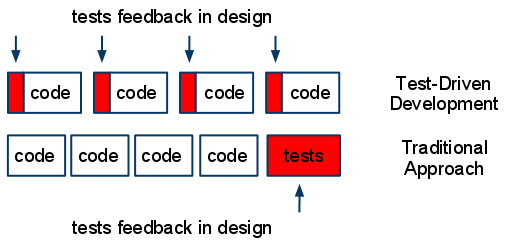
\includegraphics[scale=0.4]{tdd-and-traditional.png}
  \caption{The difference from test feedback when doing TDD or not.}
  \label{fig:tdd-feedback}
\end{figure}